\documentclass[nopagenumber,9pt]{beamer}

\mode<presentation> {
  \usetheme[]{CambridgeUS}
  %\useoutertheme{shadow}
  \setbeamercovered{transparent}
  \usecolortheme{seahorse}
%\usecolortheme{sidebartab}
%  \usefonttheme{structurebold}
  \useinnertheme{default}
\useinnertheme{rounded}
}
\usepackage{nicefrac}
\RequirePackage{amsmath,amsfonts,amsthm}
\newtheorem{Prop}{Proposition}

\usepackage{float}
\usepackage[english]{babel}
\usepackage{amsmath}
\usepackage[utf8]{inputenc}
\usepackage{times}
\usepackage{url}
\usepackage[T1]{fontenc}
%\usepackage{multirow}
\usepackage{color}
\newcommand{\mb}[1]{\mathbf{#1}}
\usepackage{graphicx}
\graphicspath{{./figure/}}
\usepackage{multirow}

\definecolor{dgreen}{RGB}{139,172,100}

\hypersetup{
  colorlinks = true,
  linkcolor = black
}
\makeatletter
\let\@mycite\@cite
\def\@cite#1#2{{\hypersetup{linkcolor=dgreen}[{#1\if@tempswa , #2\fi}]}}
\makeatother

\usepackage[ruled,vlined]{algorithm2e}
\usepackage{xcolor,colortbl}
\usepackage{rotating}
\usepackage{multirow}

\usepackage{tikz}
\usepackage{ulem}
\newcommand{\argmax}[2]{% 
\smash{\mathop{{\rm argmax}}\limits_{#1}}\,#2} 
\newcommand{\argmin}[2]{% 
\smash{\mathop{{\rm argmin}}\limits_{#1}}\,#2} 

\usepackage{stmaryrd}
\newtheorem{proposition}{Proposition}
\newcommand{\I}{\mathbb{I}}
\newcommand{\E}{\mathbb{E}}
\renewcommand{\P}{\mathbb{P}}
\newcommand{\R}{\mathbb{R}}
\newcommand{\bs}{\boldsymbol}
\newcommand{\bbeta}{\boldsymbol{\beta}}
\newcommand{\balpha}{\boldsymbol{\alpha}}
\newcommand{\btheta}{\boldsymbol{\theta}}
\newcommand{\bY}{\mathbf{Y}}
\newcommand{\bX}{\mathbf{X}}
\newcommand{\bZ}{\mathbf{Z}}
\newcommand{\by}{\mathbf{y}}
\newcommand{\bz}{\mathbf{z}}
\newcommand{\ba}{\mathbf{a}}
\newcommand{\bx}{\mathbf{x}}
\newcommand{\bh}{\mathbf{h}}
\newcommand{\bb}{\mathbf{b}}
\newcommand{\bB}{\mathbf{B}}
\newcommand{\bM}{\mathbf{M}}
\newcommand{\bphi}{\boldsymbol{\phi}}
\newcommand{\bpsi}{\boldsymbol{\psi}}
\newcommand{\bpi}{\boldsymbol{\pi}}
\newcommand{\btau}{\boldsymbol{\tau}}
\newcommand{\Ecal}{\mathcal{E}}
\newcommand{\GP}{\mathcal{GP}}
\newcommand{\bxi}{\boldsymbol{\xi}}
\newcommand{\brho}{\boldsymbol{\rho}}
\newcommand{\bgamma}{\boldsymbol{\gamma}}
\newcommand{\bsigma}{\boldsymbol{\sigma}}
\newcommand{\X}{\mathcal{X}}
\newcommand{\nf}{n_e}
\def\ee{{\mathbb E}}
\newcommand{\dd}{\mathrm{d}}

%%%macros
\newcommand{\yexpi}{y_{exp_i}}
\newcommand{\bxf}{\bx^e}
\newcommand{\byf}{\by^e}
\newcommand{\Df}{D^e}
\newcommand{\byc}{\by^c}

\newcommand{\ms}[1]{\boldsymbol{#1}}
\newcommand{\blue}{\textcolor{myblue}}
\definecolor{myblue}{RGB}{0,56,115}
\newcommand\MF{{\mathfrak{M}}}

\title[Discrepancy]{Calibration of computer models}

%titre premiere page

\subtitle{A Closer Look at the Discrepancy Function}

\author[P. Barbillon]{ Pierre \textsc{Barbillon}}
\bigskip

\date{Fall 2023}

\subject{Séminaire}



\AtBeginSection[] {
 \begin{frame}<beamer>
   \frametitle{Outline}
   \tableofcontents[currentsection]
  \end{frame}
}

\AtBeginSubsection[] {
\begin{frame}<beamer>
   \frametitle{Outline}
   \tableofcontents[currentsection,currentsubsection]
 \end{frame}
}


\begin{document}

\begin{frame}
\titlepage
%\includegraphics[scale=.12]{AgroParisTech_-_logo.PNG}
%\vspace{-1.5cm}
%\begin{flushright}
% \includegraphics[scale=.1]{Logotype-INRA-transparent.png}
% \end{flushright}
\vspace{-1cm}
\centering
\begin{tabular}{ccc}
 
\includegraphics[scale=.08]{LogoUPSaclay.jpg}&
  
\includegraphics[scale=1.3]{agrologo.png}&
   
\includegraphics[scale=.1]{LogoINRAE.jpg}
\end{tabular}


\end{frame}


\section{Validation}
\begin{frame}
Validation in \cite{bayarri2007} by examinning the Discrepancy.
tolerance bounds around the posterior predictive mean which should contain with a high probability the true real process. 
These bounds are computed by integrating the different sources of uncertainties on the simulator due to its emulation and its discrepancy with the real world process, its parameters, field data... 
The prediction for a new input variable location $\bx_{new}$ can be either a pure-simulator prediction given as 
$$\hat f(\bx_{new},\hat\btheta) = m_D(\bx_{new},\hat\btheta)$$
where $\hat \btheta$ may refer to the posterior mean or the posterior mode and $m_D$ is used instead of $f$ if we consider an expensive simulator, or a bias-corrected (discrepancy-corrected) prediction given as the mean: 
$$\hat f^R (\bx_{new})=\frac{1}{M} \sum_{j=1}^M \bigg(F^{(j)}(\bx_{new},\btheta^{(j)})+\delta^{(j)}(\bx_{new})\bigg)$$
where $F^{(j)}$ are posterior realizations of the GP $F$ given $f(D)$ (evaluations of $f$ at the DoNE) and $(\btheta^{(j)},\delta^{(j)})$ are sampled from the joint posterior predictive distribution deriving from 
Equation \eqref{eqlienrealsim} given the field data $\byf$.
For a fixed level $\gamma$, the tolerance bounds  $\tau=\tau(\bx)$ are then computed such that $\gamma\cdot 100\%$ of the samples satisfy:
$$\Big|\hat f(\bx_{new},\hat\btheta) -  m_D(\bx_{new},\hat\btheta)\Big|<\tau$$
for the pure-simulator prediction.
Similarly for the bias-corrected prediction, $\tau$ are computed such that
$\gamma\cdot 100\%$ of the samples satisfy:
$$\Big|\hat f^R (\bx_{new}) - \big(F^{(j)}(\bx_{new},\btheta^{(j)})+\delta^{(j)}(\bx_{new})\big)\Big|<\tau$$

\end{frame}


\section{Robust Calibration}
\begin{frame}
 \frametitle{$L_2$ Calibration}
 
 Defined in \cite{tuo2016theoretical}:
 $$\btheta_{L_2}=\argmin{\Theta}{\Vert \delta_{\btheta}(\cdot)\Vert_{L_2(\X)}}=\argmin{\Theta}{\bigg(\int_{\X}(\zeta(\bx)-f(\bx,\btheta))^2d\bx\bigg)^{1/2}}\,.$$


\cite{tuo2015efficient}proposes to first
obtain an estimate $\hat\zeta$ of the reality $\zeta$ via a Gaussian stochastic stochastic process and
then plug it into the minimization problem to get $\hat \btheta_{L_2}$.
Consistent estimation  $\hat \btheta_{L_2}\rightarrow\btheta_{L_2}$ provided that $\hat\zeta$ is good approximation.
 
An alternative 
least square :
$$\hat\btheta_{LS}=\argmin{\Theta}{\bigg(\sum_{i=1}^{\nf}(\yexpi-f(\bx,\btheta))^2}\bigg)\,$$
\cite{tuo2015efficient} proves the convergence $\hat \btheta_{LS}\rightarrow
\btheta_{L_2}$

\cite{wong2017} uses LS calibration as a plug-in estimator for estimating the
discrepancy function via a nonparametric regression


% Specifically, the approach in [32] estimates the reality y R (·) without the computer
% model, which contradicts the basic assumption on the usefulness of the computer model in
% reproducing the reality. On the other hand, the approach in [33] estimates θ without penalizing
% the complexity in residuals, which sometimes makes it hard to capture the residuals y R (·) −
% f M (·, θ̂ LS ) by the nonparametric regression model. A simulated example is given in Section 5.1
% to illustrate the differences between our approach and these approaches.
\end{frame}

\begin{frame}
\frametitle{Scaled Gaussian Process} 
 
 
\cite{gu2017}

\begin{align*}
 \yexpi =& f(\bx_i,\btheta)+\mu^\delta(\bx_i)+\delta_z(\bx_i)+\epsilon_i\\
 \mu^\delta=&\sum_{i=1}^q h(\bx_i)\beta_i\\
 \delta_z(\cdot)\sim&GP(0,\sigma^2_\delta c_\delta(\cdot,\cdot)) \ \text{s.t.} \ \int_{\X}\delta_z(\bx)^2d\bx=Z \\
 Z\sim & p_{\delta_z}(\cdot), \quad  p_{\delta_z}(z)\propto f_z(Z=z|\lambda  )\cdot p_{\delta}(z|\btheta,\Psi)\\
\end{align*}

where $p_{\delta}(z|\btheta,\Psi)$ is the implicit prior on $Z$ for a GP on the discrepancy.

Then if $f_z$ constant $\Rightarrow$ Model is equivalent to KOH model.



\end{frame}


\begin{frame}
 \frametitle{Comparison GP with SGP}
 \centering
 
 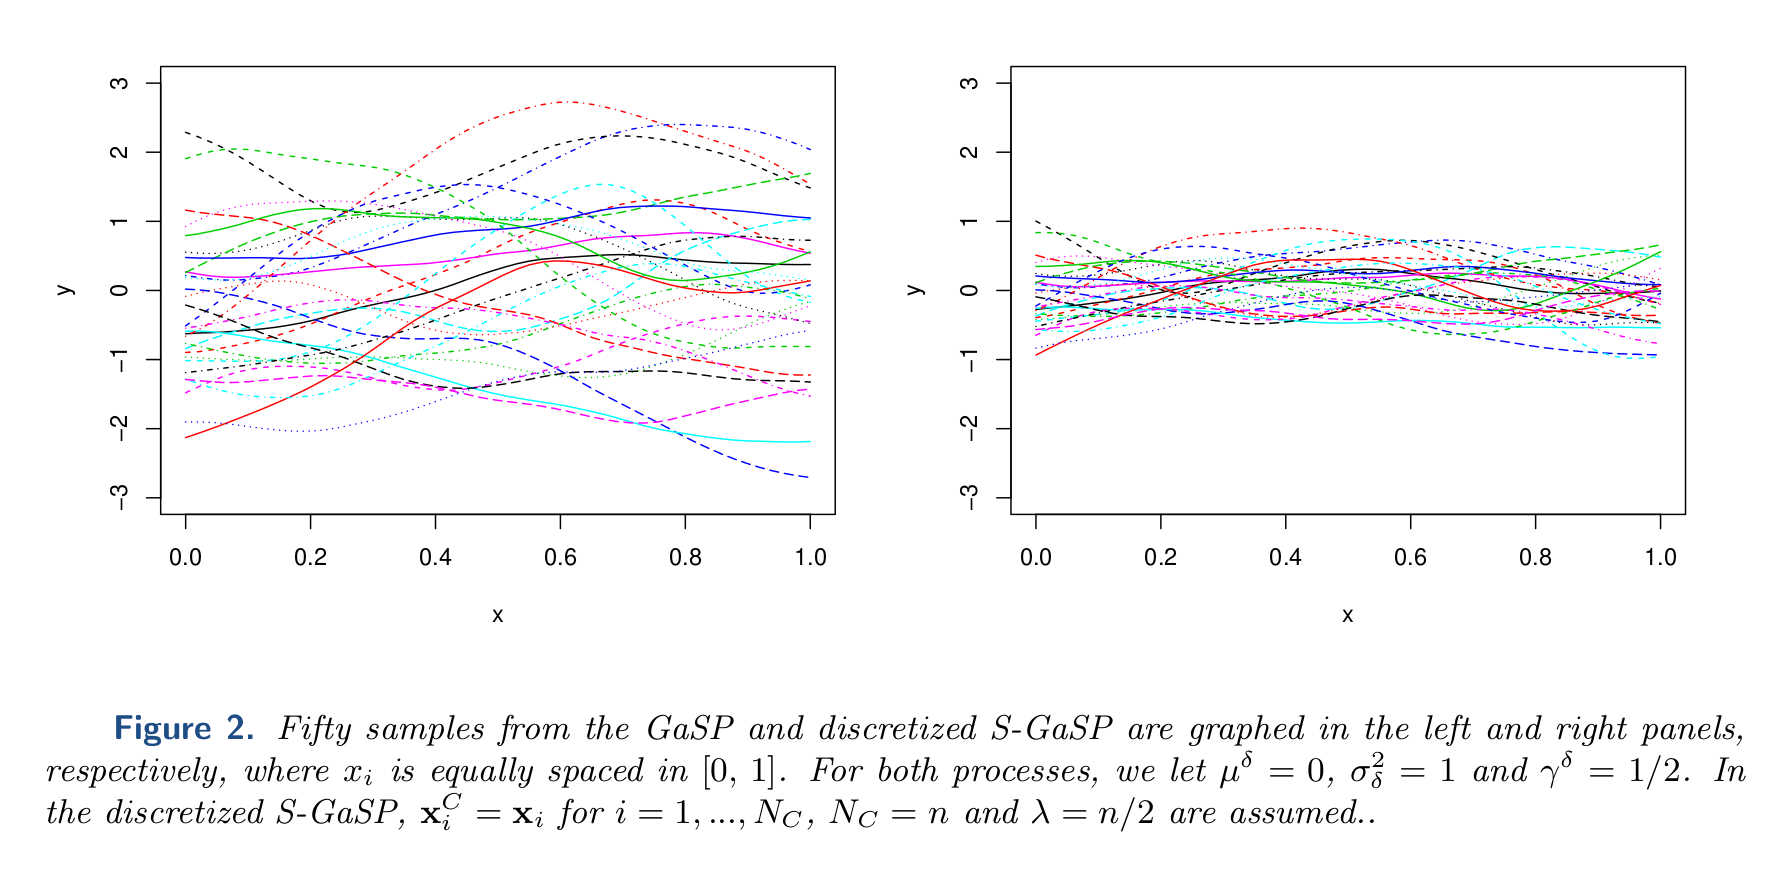
\includegraphics[scale=.2]{SGASP.png}
 
 from \cite{gu2017}.
\end{frame}



\section{Model Selection}

\subsection{Bayes Factor}
\begin{frame}
 \frametitle{Model Comparison}

 
 \begin{itemize}
  \item  $\mathcal{H}_0: \zeta(\cdot)= f(\cdot,{\btheta}^*)$ for a ``true'' $\btheta^*$:
\begin{eqnarray*}\label{eq:H0}
y_i &=& f(\bx_i,{\btheta}^*) + \epsilon^0_i\,,
\end{eqnarray*}
where $\epsilon_i^0 \overset{iid}{\sim} \mathcal{N}(0, \lambda_0^2)$.

\item[]


\item $\mathcal{H}_1:$ {\color{red} Code discrepancy} term $\delta(\bx)$ s.t.
$\zeta(\bx) = f(\bx,{\btheta}^*)+\delta(\bx) $:
 \begin{eqnarray*}\label{eq:H1}
 y_i = f(\bx_i,{\btheta}^*) + \delta(\bx_i) + \epsilon^1_i&\quad& \text{where}\quad \delta(.)\thicksim\mathcal{GP}(0,\sigma^2\Sigma_{{\psi}}(.,.))\nonumber\,\\
 &&\text{and} \quad \epsilon_i^1 \overset{iid}{\sim} \mathcal{N}(0, \lambda_1^2)
 \end{eqnarray*}

 \end{itemize}

 \bigskip
 \textbf{Bayes Factor}
  $$B_{0,1}(\bs y):=\frac
{p(\bs y|\mathcal H_0)}
{p(\bs y|\mathcal H_1)}\quad \text{where}\quad p(\bs z|\mathcal H_j) = \int_{\bs p_j} p(\bs y|\bs p_j, \mathcal H_j)\pi(\bs p_j)d \bs p_j\,.$$
  
 
\end{frame}



\begin{frame}
 \frametitle{Intrinsic Bayes Factor}
 
 {\color{blue} Berger and Perrichi (1996)}.\\
 
 \medskip
{{ Main issue:}} Evidence $p(\bs y|\mathcal{H}_j)${ sensitive to priors} $\pi(\bs p_j)$.

\begin{itemize}
\item Need to use { compatible priors} {\color{blue} Celeux et al. (2006)} or { objective priors} {\color{blue} Casella (2006)}, 
\item but marginal likelihood {{ ill-defined}} (up to arbitrary constant) for {{ improper priors}} (as {{ objective priors}} often are).
\end{itemize}


\blue{Idea:} using a part of data to obtain a proper prior:

\begin{itemize}
 \item Partial Bayes Factor:



\begin{eqnarray*}\label{eq:partialBF}
B_{0,1}(\bs y(-m)|\bs y(m)) 
&=& 
\frac{\int l(\bs p_0 ;\bs y(-m)|\bs y(m)) \pi(\bs p_0|\bs y(m))d\bs p_0}{\int l(\bs p_1 ;\bs y(-m)|\bs y(m)) \pi(\bs p_1|\bs y(m))d\bs p_1}
=
\frac
{B_{0,1}(\bs y)}
{B_{0,1}(\bs y(m))}\,.
\end{eqnarray*}
\item $B_{0,1}(\bs y(-m)|\bs y(m))$ {\blue{ well-defined}} for $|m|\geq n_0$ large enough:

\item { Intrinsinc Bayes factor} obtained by averaging over all $\bs y(m)$s :
\begin{eqnarray*}\label{eq:AIF}
B_{0,1}^A(\bs y) &=& \frac{B_{0,1}(\bs z)}{C(n,n_0)} \sum_{|m|=n_0} B_{0,1}(\bs y(m))^{-1} \,.
\end{eqnarray*}
\end{itemize}

 
\end{frame}



\begin{frame}
 
\frametitle{IBF computation under linearization of the code}
{\bf{ Linear assumption}}: 
$f(\bs x,\bs \theta)=g(\bs x)^\top\bs\theta$,
with $g(\bs x)\in\mathbb R^d$.
  
\smallskip
{\bf{ Prior choices and consequences}}: 
\begin{itemize}
	\item Model~$\mathcal{H}_0$ boils down to:
	\begin{eqnarray*}
	\mathcal H_0: \bs y &\sim& 
	\mathcal N({ G}\bs\theta_0; \lambda_0^2\rm I_n);\quad \bs p_0 = (\bs\theta_0, \lambda_0^2)
	\end{eqnarray*}
	where ${ G}=[g(\bs x_1),\cdots,g(\bs x_n)]^\top \text{the}\ n\times p\ \text{design matrix.}$
	\begin{itemize}
		\item[$\hookrightarrow$] Under Jeffreys prior: $\pi(\bs p_0)\propto\lambda_0^{-2}$, $p(\bs y|\mathcal H_0)$  explicit.
	\end{itemize}
	\item Model~$\mathcal H_1$ boils down to:
	\begin{eqnarray*}
	\mathcal H_1: \bs y &\sim& 
	\mathcal N( G\bs\theta_1; \sigma^2 V_{k,\psi});\quad
	%\mathcal N( G\bs\theta_1; \sigma^2\left(k\rm I_n+\Sigma_\psi\right));\quad
	\bs p_1 = (\bs\theta_1, \sigma^2,\psi,k) 
	\\&&\quad V_{k,\psi}(i,j) =k\delta_{i,j}+e^{-||\bs x_i - \bs x_j||^2/\psi^2}
	\quad k=\lambda_1^2\sigma^{-2}\,.
	\end{eqnarray*}

	%$\Sigma_\psi(i,j)=e^{-||\bs x_i - \bs x_j||^2/\psi^2}$ and  
	\begin{itemize}
		\item Prior choice: $\pi(\bs p_1)\propto \pi(\psi|k)\pi(k)\sigma^{-2}$ {\color{blue} Berger et al. (2001)} with proper priors for $\pi(\psi|k)\pi(k)$,
		\item Integration of $p(\bs y|\bs p_1,\mathcal H_1)$: {{ explicit}} over $(\theta_1, \sigma^2)$, by {{ Gaussian quadrature}} over $(\psi,k)$.
	\end{itemize}
\end{itemize}

 
\end{frame}




\begin{frame}
 \frametitle{Computation of the IBF}
 
 \begin{beamerboxesrounded}{Proposition}
  If $\pi(\bs p_1)=\pi(\theta_1,\sigma^2,\psi,k)=\pi(\psi|k)\pi(k)/\sigma^2$, $\pi(\psi,k)$ is proper and $m=d+1$ then
  $$B_{0,1}^A(\bs y)=\frac{B_{0,1}(\bs z)}{C(n,n_0)} \sum_{|m|=n_0} B_{0,1}(\bs y(m))^{-1}=B_{0,1}(\bs y)$$
 \end{beamerboxesrounded}

 \bigskip
 
 Proof: Consequence of \color{blue}Berger et al. (1998)\color{black}.
 
 \bigskip
 
 In the following, 
 \begin{eqnarray*}
  \pi(\psi|k)&=& \mathcal{U}([0,1])\,, \\
  \pi(k)&=&Be(1,3)\,.
 \end{eqnarray*}

 
 
\end{frame}





\begin{frame}
 \frametitle{Synthetic data}
  
  
  Data simulated according to model~$\mathcal{H}_1$, with $\delta\sim GP(0,\sigma^2\Sigma_\psi)$:
$$
\bs x = \left(\frac i n \right)_{1\leq i\leq n},\quad n=30,\quad\sigma^2=0.1,\quad k=0.1\,.
$$
From left to right
\begin{itemize}
\item constant trend $g(\bx)=1$ ; $\theta_1=1$, 
\item linear trend $g(\bx)=(1,x)$ ; $\bs{\theta}_1=(1,1)$,
\item quadratic trend $g(\bx)=(1,x,x^2)$ ; $\bs{\theta}_1=(1,1,1)$.
\end{itemize}
\begin{itemize}
\item Bayes factor $B_{0,1}^A$ expected to {{ decrease} with $\psi$}.
\end{itemize}

\begin{center}
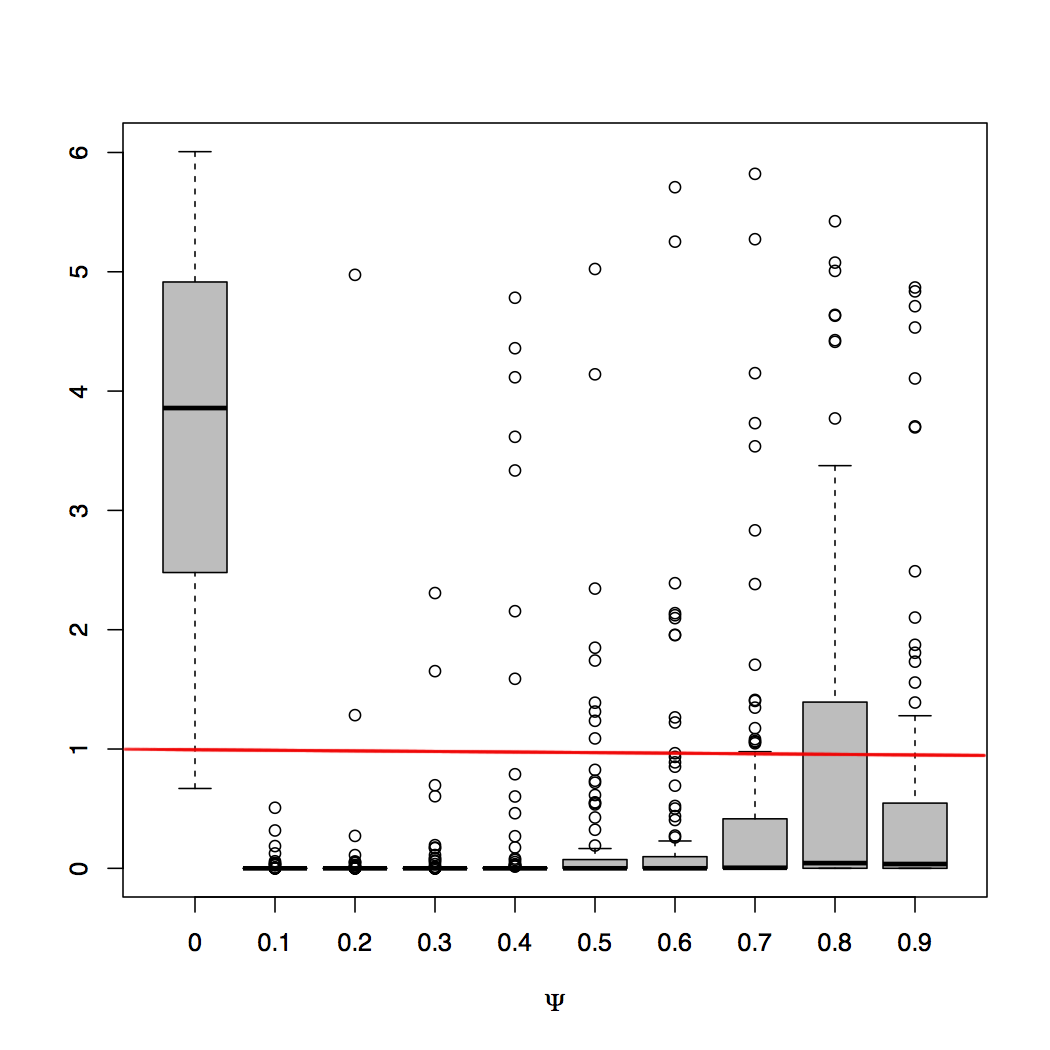
\includegraphics[width=0.2\textwidth]{const_30_unif_prior.png}
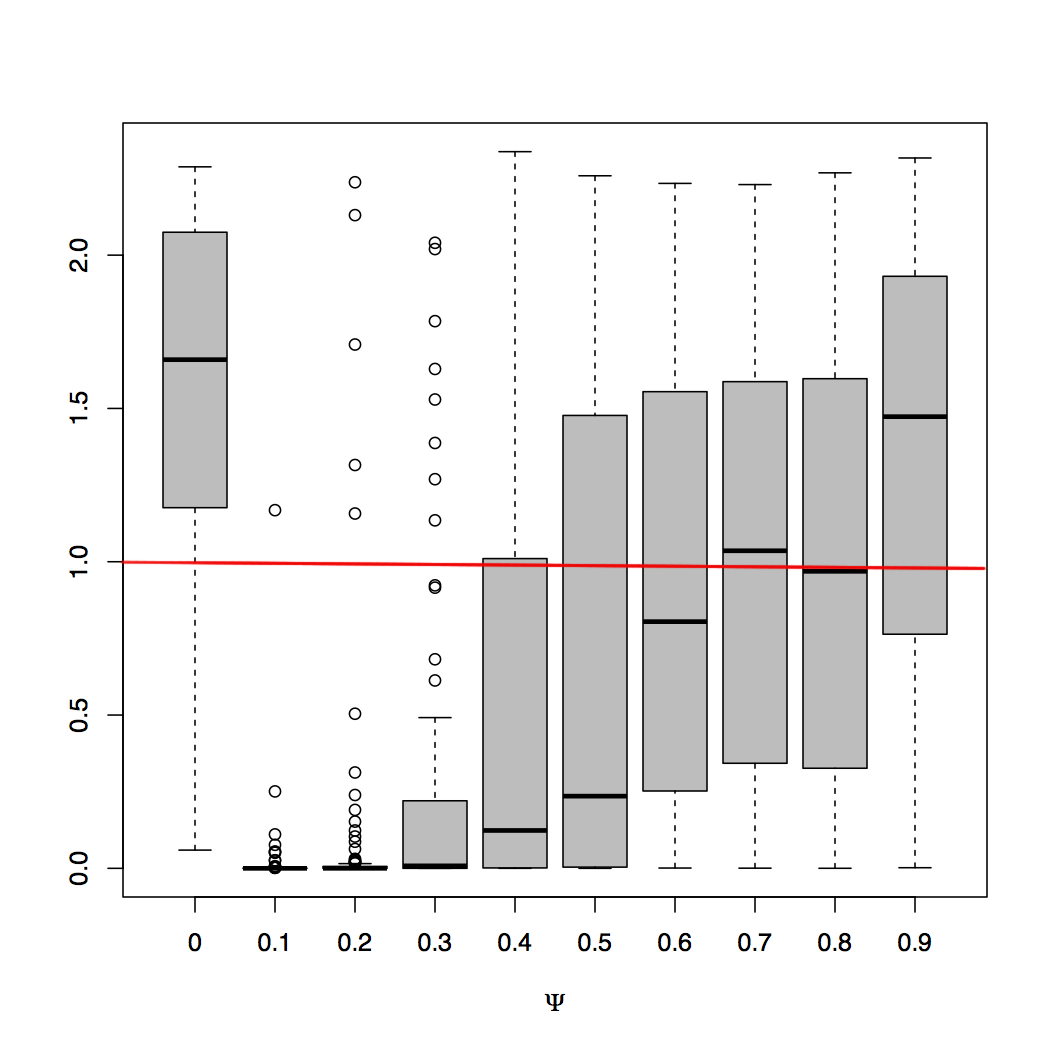
\includegraphics[width=0.2\textwidth]{lin_30_unif_prior.png}
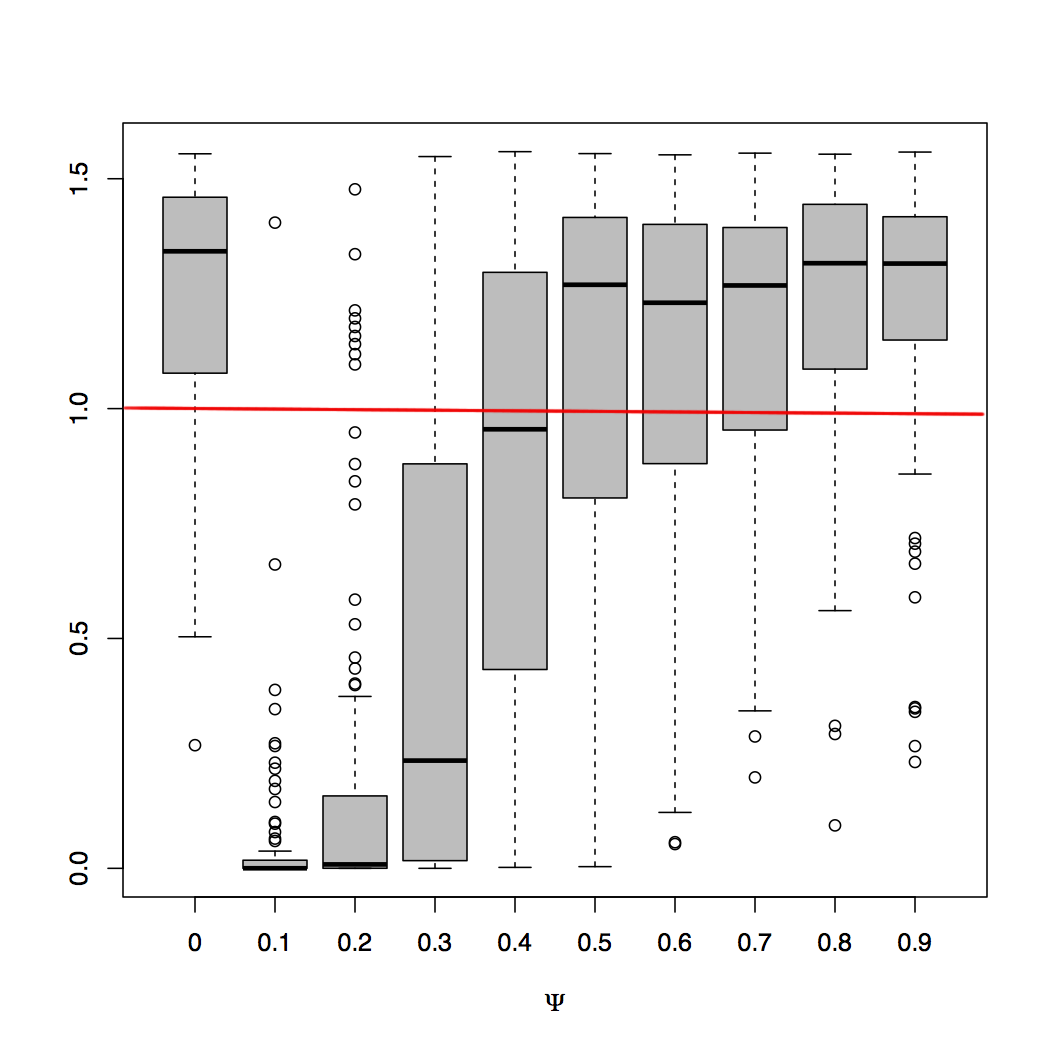
\includegraphics[width=0.2\textwidth]{poly_30_unif_prior.png}

Boxplots of $B_{0,1}^A(\bs y)$ values over $100$ simulations with constant, linear and quadratic trends (left to right)
\end{center}

% \begin{itemize}
% 
% \item $\mathcal H_0$ selected over $\mathcal H_1$ if $B_{0,1}^A(\bs z)>1$.
% \item Due to the confounding between non-constant trend and discrepancy, $\mathcal H_0$ and $\mathcal H_1$ {\color{red} hard to distinguish for $\psi > 0.3$}.
% \end{itemize}


\end{frame}


\begin{frame}
\frametitle{Confounding Effect}


% 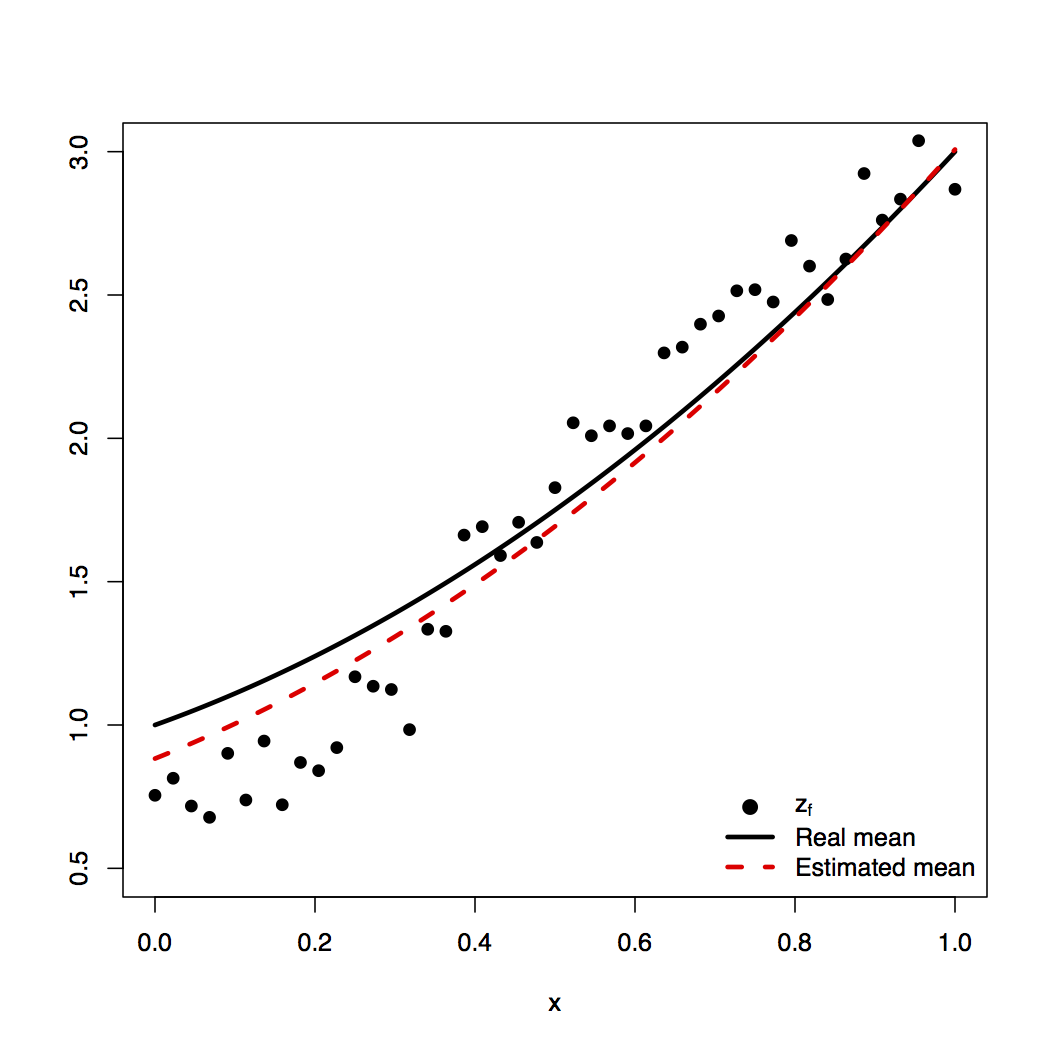
\includegraphics[width=.15\textwidth]{Confounding_0_2.png}
% 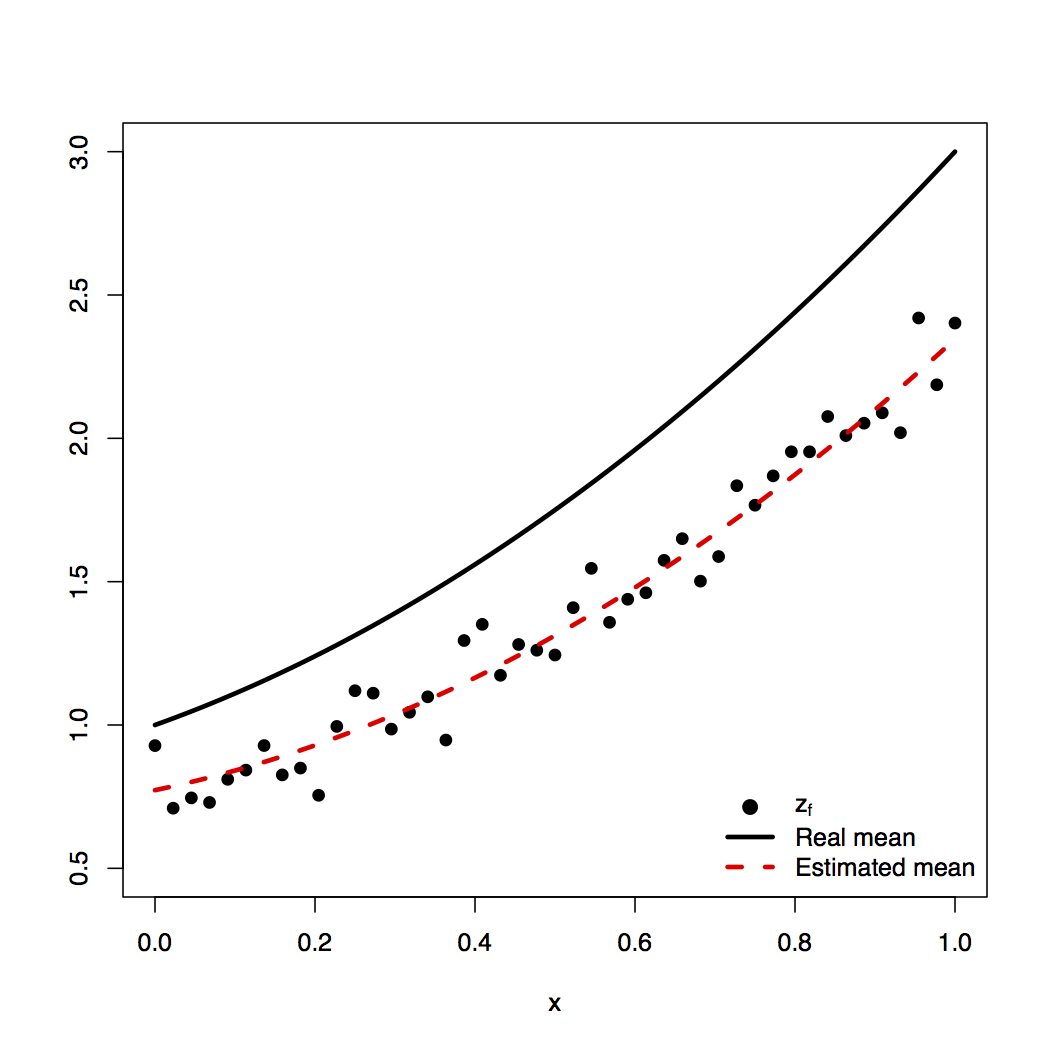
\includegraphics[width=.15\textwidth]{Confounding_0_7.png}\\
%      $\psi=.2$  $\psi=0.7$

\begin{center}
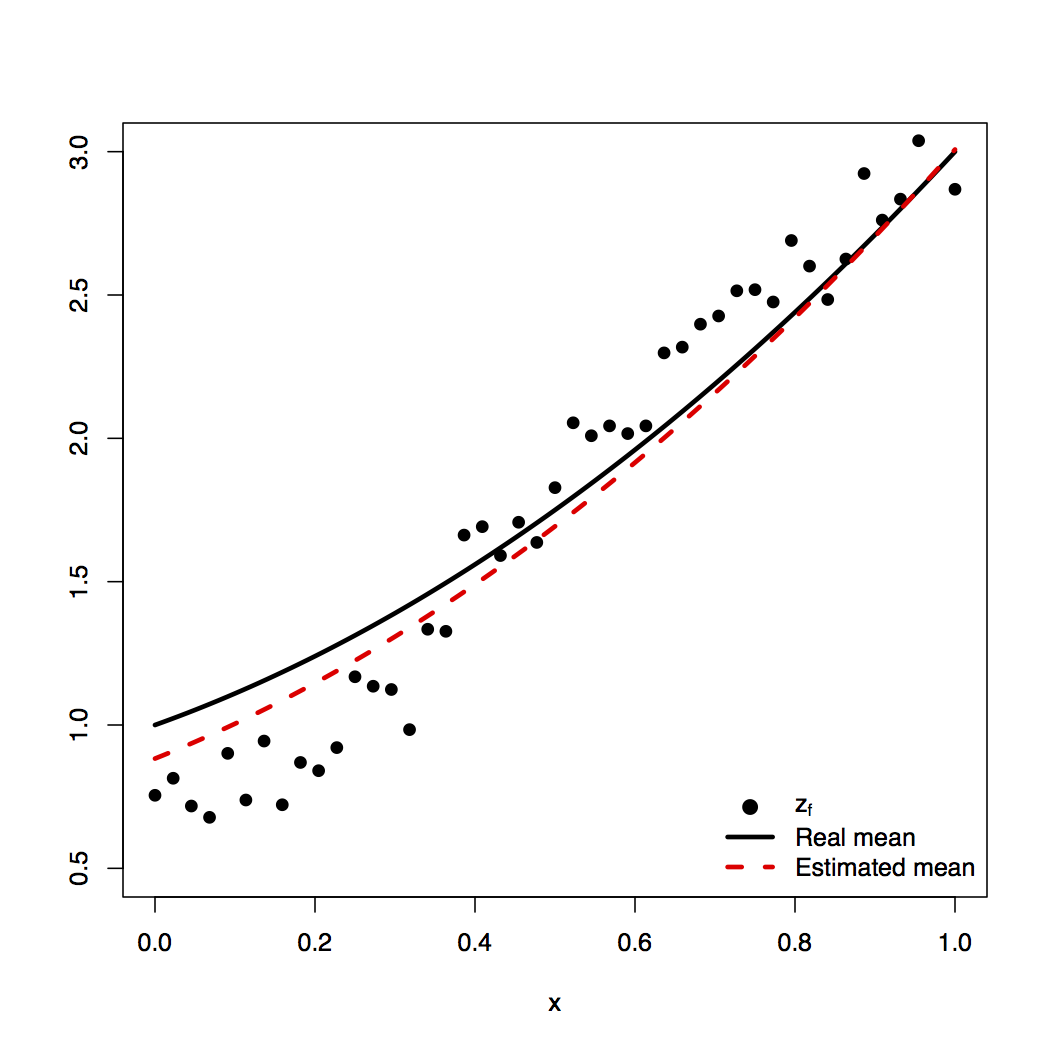
\includegraphics[width=.4\textwidth]{Confounding_0_2.png}
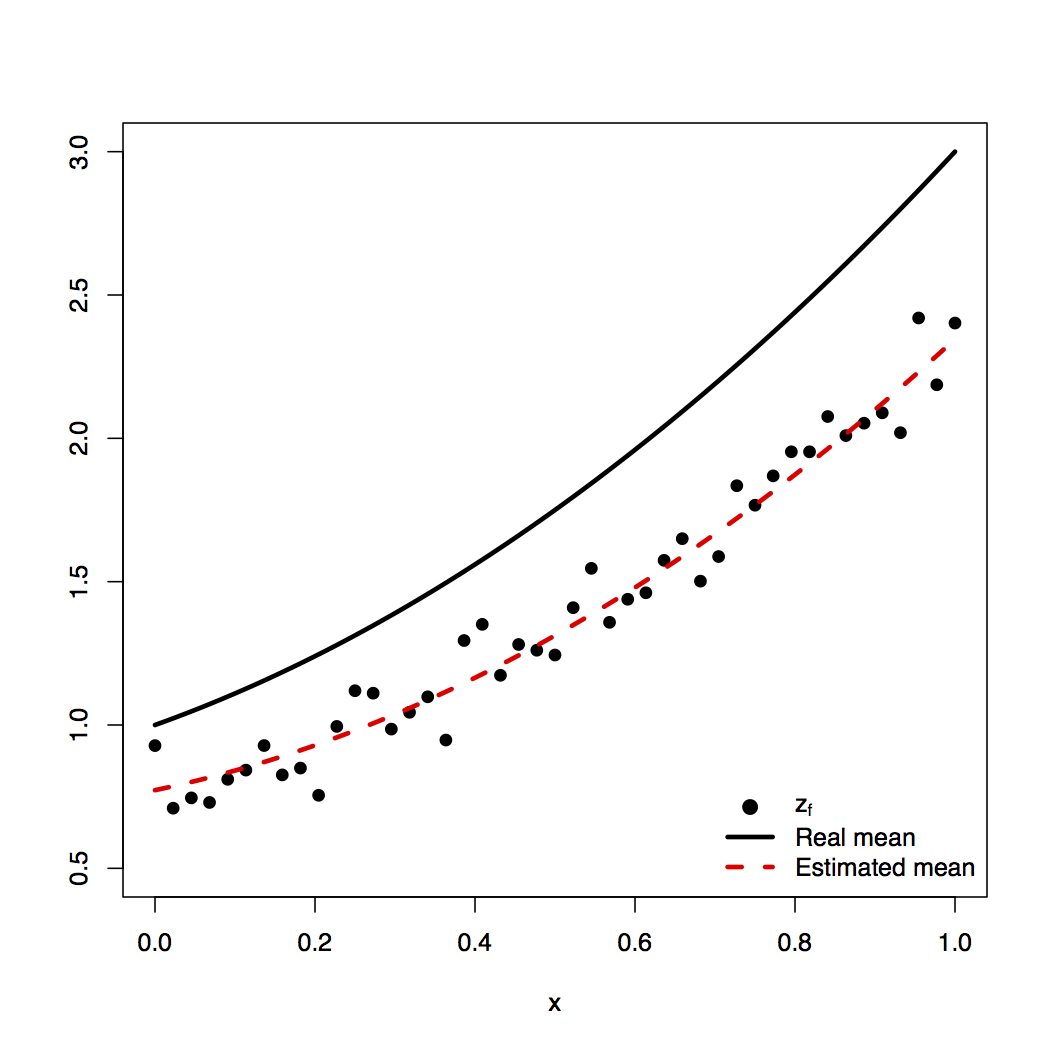
\includegraphics[width=.4\textwidth]{Confounding_0_7.png}\\
 $\psi=0.2$ left and $\psi=0.7$ right
 \end{center}

  
     
\begin{itemize}
%\item Data simulated with quadratic trend and $\psi \in \{0.2, 0.7\}$
\item $\psi,k,\sigma^2$ estimated by maximum likelihood.
\item For $\psi=0.7$, discrepancy indistinguishable from quadratic trend!
\end{itemize}
  
 
\end{frame}


\begin{frame}
 \frametitle{Case description}
\begin{itemize}
\item Industrial computer code predicting the \blue{\bf productivity} of an electric power plant, based on measurements (temperature, pressure, discharge, \ldots)  throughout the plant
%\item Code used periodically to detect \red{\bf power loss} and diagnose probable causes
%\item Validation of the computer code crucial to ensure \blue{\bf early detection} and \blue{\bf correct identification} of causes
\item $n=24$ available field measures (results of periodic testing) to validate code
\end{itemize}
Main code features:
\begin{itemize}
\item $p=20$ input variables ($\bs x \in \mathbb R^{20}$)
\item $d=2$ parameters: heat transfer coefficient of the condenser, yield of the main turbine 2 .
\item Two outputs of interest (electric power, condenser pressure), seen here as two separate codes 
\item Code \blue{\bf linearized} in neighbourhood of reference value $\theta^\star$:
\begin{eqnarray*}
f(\bs x_i,{\bs \theta}) \approx f(\bs x_i,\bs \theta^\star) + h(\bs x_i)^\top (\bs \theta-\bs \theta^\star),
\end{eqnarray*}
where $h(\bs x_i) = \nabla_{\bs \theta} f(\bs x_i,\bs \theta^\star)$ evaluated numerically through finite difference
\end{itemize}

\end{frame}


\begin{frame}
 \frametitle{Calibrated code predictions vs measures}
\begin{minipage}{.5\textwidth}
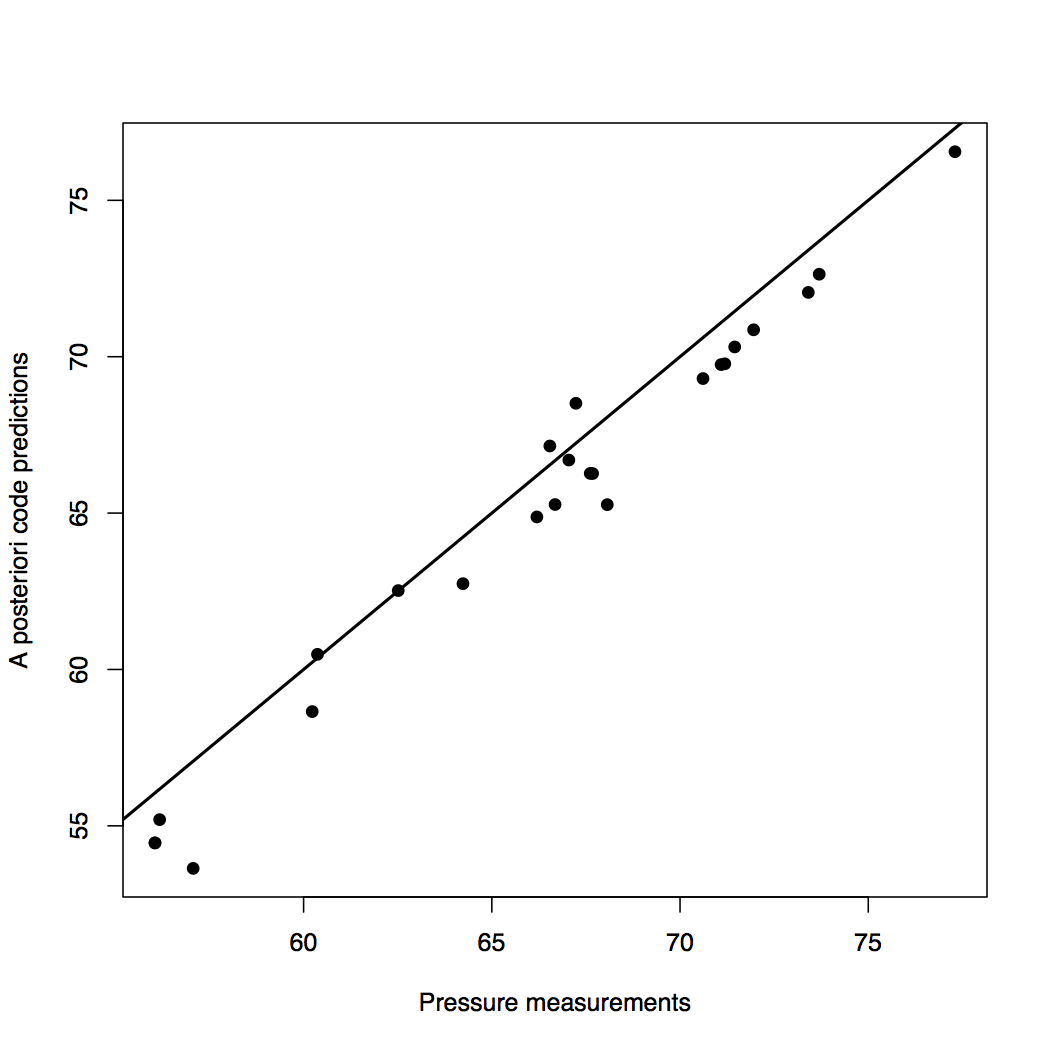
\includegraphics[width=\textwidth]{code_post_vs_measure_P.png}\\
\centering Pressure \\
$B_{0,1}^A=2\times10^{-18}$ 
\end{minipage}\hfill
\begin{minipage}{.5\textwidth}
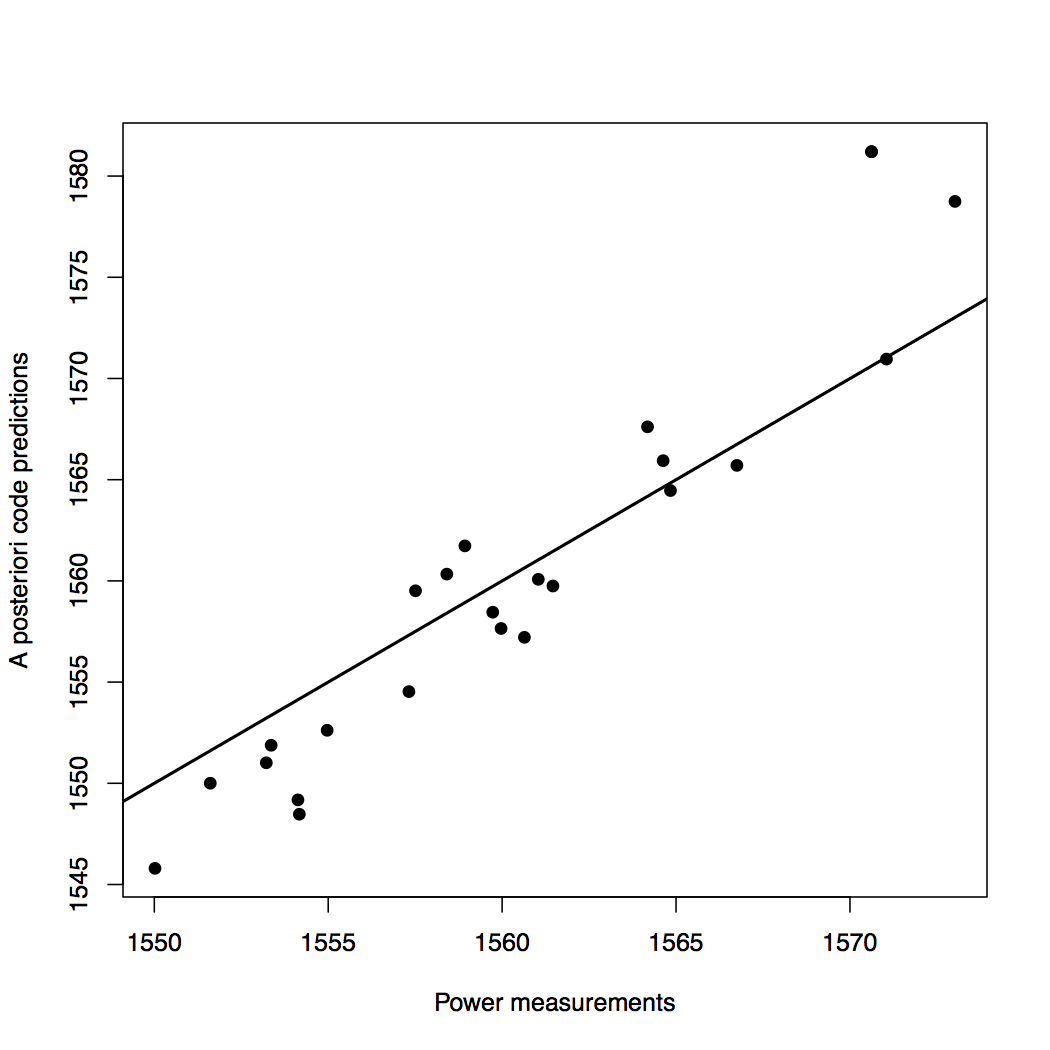
\includegraphics[width=\textwidth]{code_post_vs_measure_W.png}\\
\centering Power \\
$B_{0,1}^A=3\times10^{-3}$ 
\end{minipage}
\begin{itemize}
\item Bias reduced by calibration, but not supressed
\item strong evidence for code discrepancy 
\end{itemize}
 
\end{frame}








\subsection{Mixture model}

\begin{frame}
 \frametitle{Model selection as a mixture problem}
\color{blue}Kamary et al. (2014)\color{black}
 
 
 Model selection problem:
 \begin{align}\label{eq:2}
\MF_0: y_i&=f(\bx_i, \pmb{\theta}_0)+\epsilon_i^0 \nonumber\\
\MF_1: y_i&=f(\bx_i, \pmb{\theta}_1)+\delta(\bx_i)+\epsilon_i^1.\nonumber
\end{align}
where $\epsilon_i^0 \overset{iid}{\sim} \mathcal{N}(0, \lambda_0^2)$ and $\epsilon_i^1 \overset{iid}{\sim} \mathcal{N}(0, \lambda_1^2)$

\medskip

converted into a mixture model:
\begin{equation*}\label{eq:1}
\MF_\alpha: y_i\sim \alpha \left(\ell_{\MF_0}(\pmb{\theta}_0, \lambda_0^2;y_i, \bx_i)\right)+(1-\alpha)\left(\ell_{\MF_1}(\pmb{\theta}_1, \lambda_1^2, \delta;y_i, \bx_i)\right)\,.
\end{equation*}

 
 
 \medskip
 \begin{itemize}
  \item Model $\MF_\alpha$ is defined under the hypothesis that the likelihood of the model $\MF_1$ is conditioned on $\delta$.
  \item  $\delta$ is considered as a parameter of $\MF_1$.
  \item Conditionnally on $\delta$, the $y_i$'s are considered  independent.
  \item Posterior distribution on $\alpha$ will provide a decision rule for $\MF_0$ against $\MF_1$.
 \end{itemize}
\end{frame}



\begin{frame}
 \frametitle{Hypotheses and prior distribution}
 
 \begin{itemize}
 
 \item Linear code: $f(\bx,\pmb{\theta})=g(\bx)\pmb{\theta}$.
 \bigskip
 
 \item GP prior for discrepancy function:
 $$\delta(.)\thicksim\mathcal{GP}(0,\sigma^2\Sigma_{{\psi}}(.,.))\,.$$
 
 \bigskip
 
 \item Some parameters are common, $\btheta$ and $\lambda^2$ so a common prior distribution is chosen for both.
 
 
 \begin{equation*}\label{eq:1}
\MF_\alpha: y_i\sim \alpha \left(\ell_{\MF_0}(\pmb{\theta}, \lambda^2;y_i, \bx_i)\right)+(1-\alpha)\left(\ell_{\MF_1}(\pmb{\theta}, \lambda^2, \delta;y_i, \bx_i)\right)\,.
\end{equation*}

 
 \end{itemize}

 

 
 \end{frame}

 
 
 \begin{frame}
  \frametitle{Posterior distribution}
  
   \begin{beamerboxesrounded}{Theorem}
Let $g: \mathbb{R}^p \to \mathbb{R}^d$ be a finite-valued function and vector $x_1,\ldots,x_n$ such that the rank of $\{g(x_1),\ldots,g(x_n)\}$ is $d$.
%$g^T(x_i)g(x_i)$ be a positive-definite matri2x when $i=1, \ldots, n$. Suppose also that for any sample size $n$, there exists a function such as $g^{-1}()$ for which we have $g(x_i)g^{-1}(x_i)=1$. 
The posterior distribution associated with the prior $\pi(\pmb{\theta}, \lambda^2)=\nicefrac{1}{\lambda^2}$ and with the likelihood is proper when
\begin{itemize}
\item for any $0<k<1$, the hyperparameter $\sigma^2$ of the discrepancy prior distribution is reparameterized as $\sigma^2=\nicefrac{\lambda^2}{k} $ and so $\Sigma_\psi=(\nicefrac{\lambda^2}{k})  \text{Corr}_{\psi_\delta}$ when $\text{Corr}_{\psi_\delta}$ is the correlation function of $\delta$. %This reparameterization essentially implies that the variance of the computer model discrepancy is a priori supposed to be larger than the variance of the field measurement white noise; %(une phrase \`a rajouter pour dire que pour quoi $0<k<1$ ? C'est quoi l'int\'er\^et de cette hypoth\`ese dans le contexte du mod\`ele avec le biais?)
%\item prior for $\lambda$ is a maximum entropy probability defined as $\pi(\lambda)\propto \nicefrac{1}{\lambda}\exp(\nicefrac{-\beta}{\lambda})$ with $\mathbf{E}_{\lambda}(\nicefrac{1}{\lambda})=\nicefrac{1}{\beta}$ and $\beta$ known;
%\item the dimensionality, $d$, is less than $n$;% 
\item the mixture weight $\alpha$ has a proper beta prior $\mathcal{B}(a_0, a_0)$; 
\item $\psi_\delta$ has a proper Beta prior $\mathcal{B}(b_1, b_2)$.
\item proper distribution is used on $k$.
\end{itemize}

 \end{beamerboxesrounded}

 \end{frame}

 
 

 
 \begin{frame}
  \frametitle{Metropolis within Gibbs}
  
   \tiny{
 \begin{algorithm}[H]
  \SetSideCommentLeft
  \DontPrintSemicolon
  \For{t=1,\ldots,T}{  
  \begin{description}
\item[a)] %For each MCMC iteration $t$, $t=1,\ldots,T $, 
$\delta^{(t)}$ is sampled from $\pi(\delta|\pmb{y},\bx,\pmb{\theta}^{(t-1)},\lambda^{(t-1)},k^{(t-1)},\psi_\delta^{(t-1)},\alpha^{(t-1)})$ as follows.%through the two-steps.
\begin{description}
\item[a.1)] For $i=1, \ldots, n; j=0,1$, generate auxiliaire variable $\zeta_i^{(t)}$ from 
$$\mathbb{P}(\zeta_i=j|y_i,x_i,\delta^{(t-1)},\pmb{\theta}^{(t-1)},\lambda^{(t-1)},k^{(t-1)},\psi_\delta^{(t-1)})\,.$$
 %defined in \eqref{zeta}. 
\item[a.2)] Generate $\delta^{(t)}$ according to the conditional posterior distribution 
$$\delta^{(t)}|\pmb{y},\bx,\zeta^{(t)}=1,\pmb{\theta}^{(t-1)},\lambda^{(t-1)},k^{(t-1)},\psi_\delta^{(t-1)},\alpha^{(t-1)}\sim\mathcal{N}_{n}(\hat{\mu}_\delta, \hat{\Sigma}_\delta)\,.$$
%with $\hat{\mu}_\delta, \hat{\Sigma}_\delta$ defined in \eqref{musigdlt}.
\end{description}
\item[b)] Generate $\pmb{\theta}^{(t)}|\pmb{y}, \bx, \pmb{\zeta}^{(t)}, \delta^{(t)}, \lambda^{(t-1)}, k^{(t-1)}, \alpha^{(t-1)} \sim\mathcal{N}_d(\hat{\mu}_{\pmb{\theta}}, \hat{\Sigma}_{\pmb{\theta}})$.
\item[c)] Generate $\lambda^{(t)}|\pmb{y}, \bx, \pmb{\zeta}^{(t)}, \delta^{(t-1)}, \pmb{\theta}^{(t)}, k^{(t-1)}, \alpha^{(t-1)} \sim \mathcal{IG}(\hat{a}_\lambda, \hat{b}_\lambda)$.
\item[d)] Generate $\alpha^{(t)}|\pmb{y}, \bx, \pmb{\zeta}^{(t)}, \delta^{(t)}, \pmb{\theta}^{(t)}, \lambda^{(t)}, k^{(t-1)}\sim \mathcal{B}eta(n-m+a_0, m+a_0)$.
\item[e)] Generate $k^{(t)}$ from a random walk Metropolis-Hastings algorithm conditionally to $(\pmb{y}, \bx, \pmb{\zeta}^{(t)}, \delta^{(t)}, \pmb{\theta}^{(t)}, \lambda^{(t)},\alpha^{(t)}, \psi_\delta^{(t-1)})$.
\item[f)] Generate $\psi_\delta^{(t)}$ from a random walk Metropolis-Hastings algorithm conditionally to $(\pmb{y}, \bx, \pmb{\zeta}^{(t)}, \delta^{(t)}, \pmb{\theta}^{(t)}, \lambda^{(t)}, \alpha^{(t)},k^{(t)})$.
\end{description}
  }
  \caption{Metropolis-within-Gibbs algorithm}
 \label{algo:mwg}
\end{algorithm}
}
  
 \end{frame}

 
 
 \begin{frame}
  \frametitle{Synthetic example $\MF_0$}
  Code is a quadratic function.\\
  $50$ datasets of size $n=30$ from $\MF_0: y_i=g(x)\pmb{\theta}^*+\epsilon_i$. \\
  Priors as in the theorem, $\alpha\sim \mathcal{B}eta(1,1)$, $\delta\sim \mathcal{GP}(0_n, \Sigma_\psi)$, $\psi_\delta \sim \mathcal{B}eta(1,1)$ and  $k \sim \mathcal{B}eta(1,1)$.  \\
  Number of MCMC iterations is $10^4$ with a burn-in of $10^3$ iterations
  
\begin{figure}[ht]
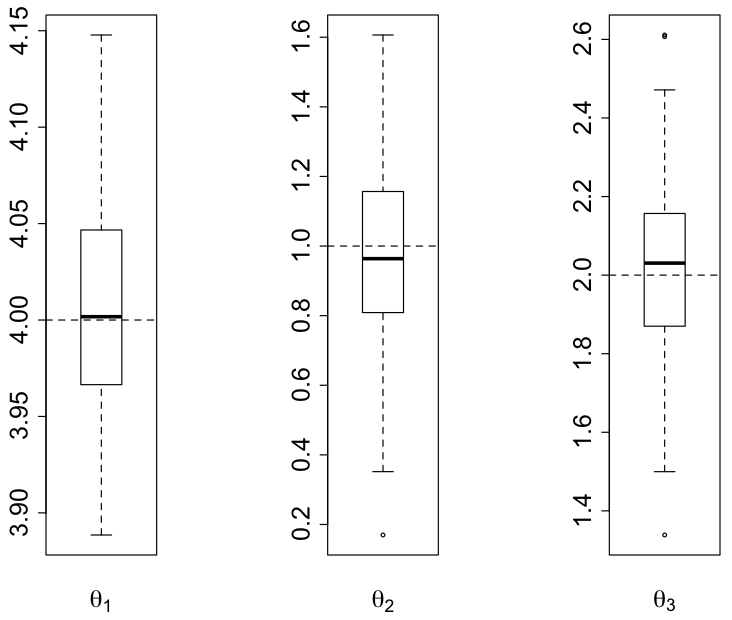
\includegraphics[width=0.2\textwidth,height=4cm]{m0_theta_50data_n_30_gamadelta_0_9}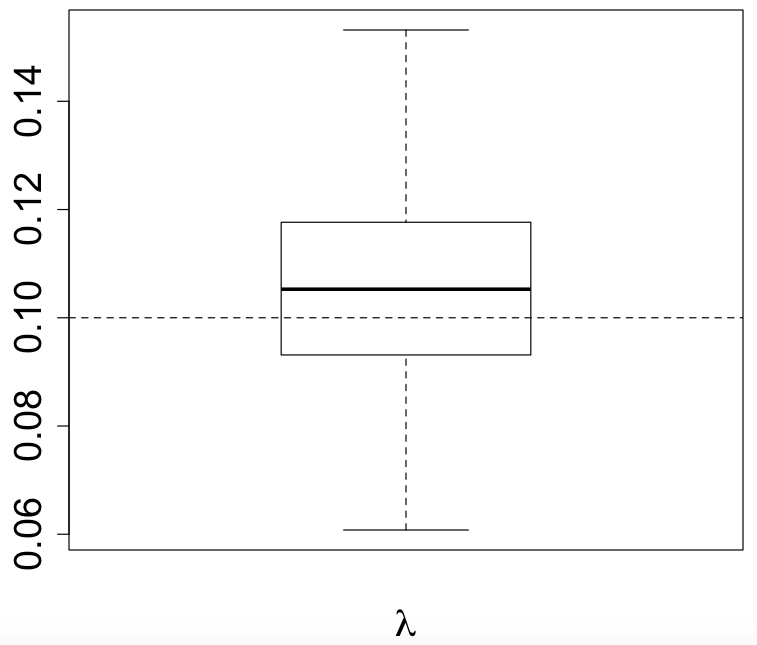
\includegraphics[width=0.2\textwidth,height=4cm]{m0_lamda_50data_n_30_gamadelta_0_9}
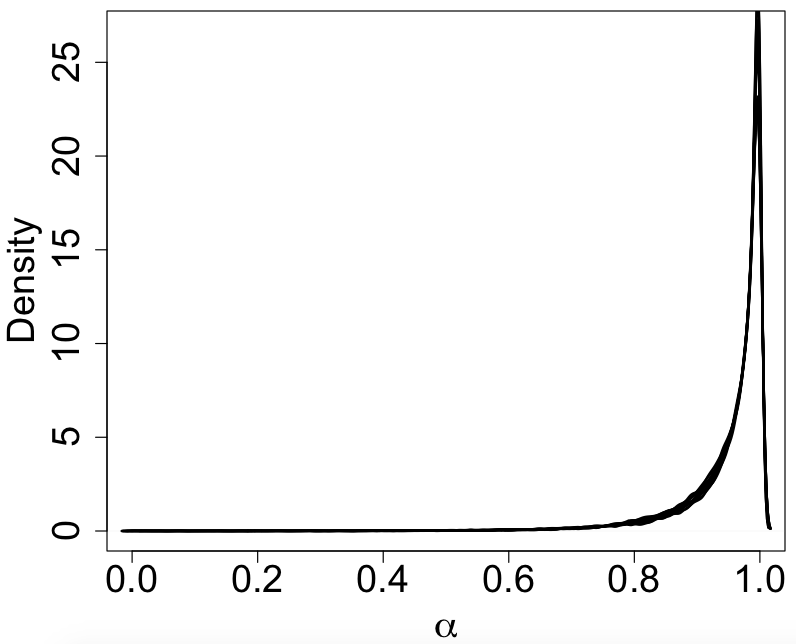
\includegraphics[width=0.2\textwidth,height=4cm]{m0_alpha_50data_n_30_gamadelta_0_9}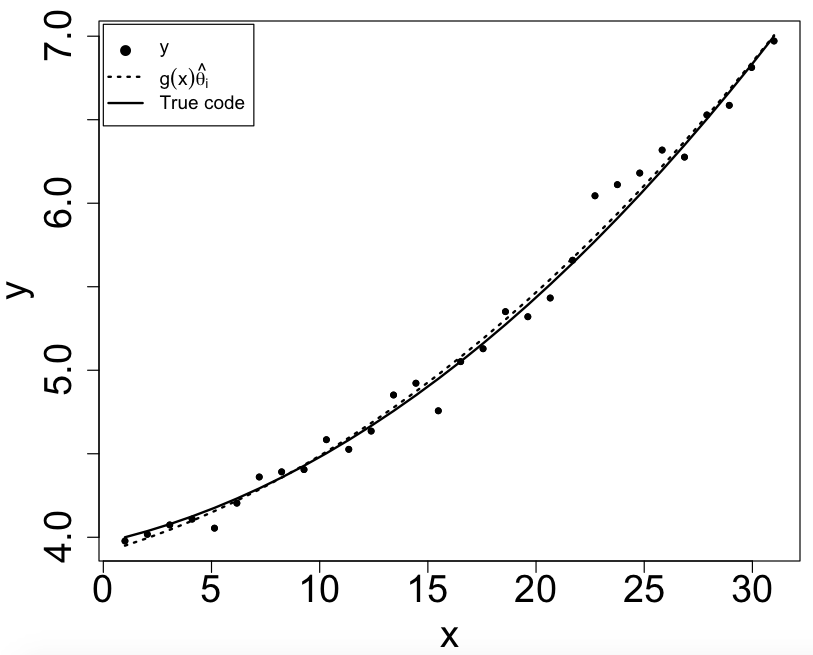
\includegraphics[width=0.2\textwidth,height=4cm]{m0_model_50data_n_30_gamadelta_0_9}
\caption{Posterior mean estimates of $\btheta,\lambda^2$, Posterior densities of $\alpha$, Posterior prediction of the code.}
  \end{figure}

 \end{frame}



  \begin{frame}
  \frametitle{Synthetic example $\MF_1$}
  Code is a quadratic function.\\
 $50$ samples of size $50$ simulated from $\MF_1$ when $\psi_\delta^*$ varies between $0.01$ and $0.9$, $\delta^*(x)\sim \mathcal{GP}(0_n, \Sigma_\psi)$, $ \lambda^2*=0.1$ and $k^*=0.1$.\\
  Priors as in the theorem, $\alpha\sim \mathcal{B}eta(1,1)$, $\delta\sim \mathcal{GP}(0_n, \Sigma_\psi)$, $\psi_\delta \sim \mathcal{B}eta(1,1)$ and  $k \sim \mathcal{B}eta(1,1)$.  \\
 Number of MCMC iterations is $10^4$ with a burn-in of $10^3$ iterations.
%  Figure \ref{figure:m1_1} illustrates  that the posterior means of $\alpha$ are close to zero when $\psi_\delta^*\geq 0.1$. This means that the true model $\MF_1$ is supported by $\alpha$ for the data in this case. %On the other hand, when the prior of the correlation length is informative and $\psi_\delta^*=0.01, 0.05$ and $0.1$, $\alpha$ is close to zero in favour of the true model $\MF_1$. 
% The increase of the means of $\alpha$ is however illustrated by the figure when $\psi_\delta\in (0,0.1)$. On the other hand, $\lambda$ is overestimated when $\psi_\delta<0.1$ and the more $\psi_\delta$ increases, the more $\lambda$ tends to the true value $0.1$. For both correlation length priors, the posterior estimates of $\alpha$ and $\lambda$ have almost the same behaviors.



\begin{figure}[ht]
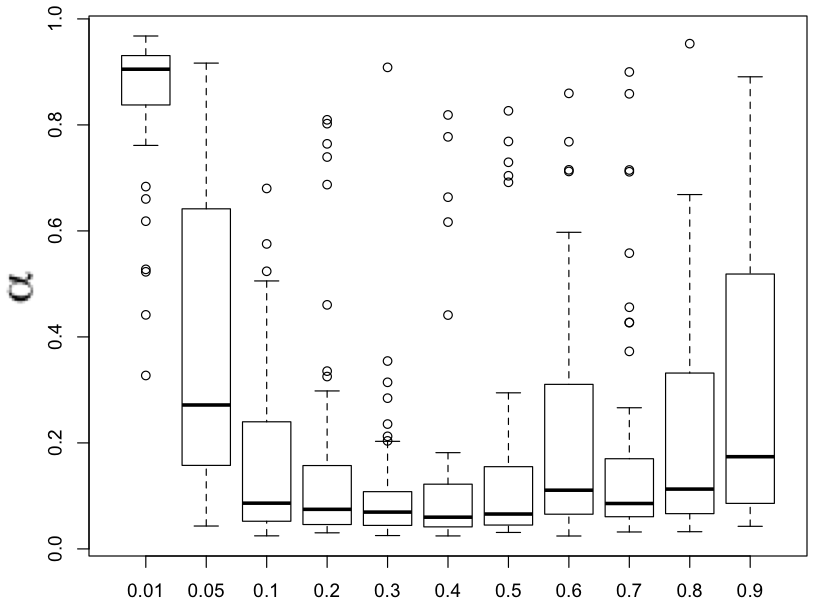
\includegraphics[width=0.4\textwidth]{100data_alpha_n_50_m1_uniform_gamadelta}
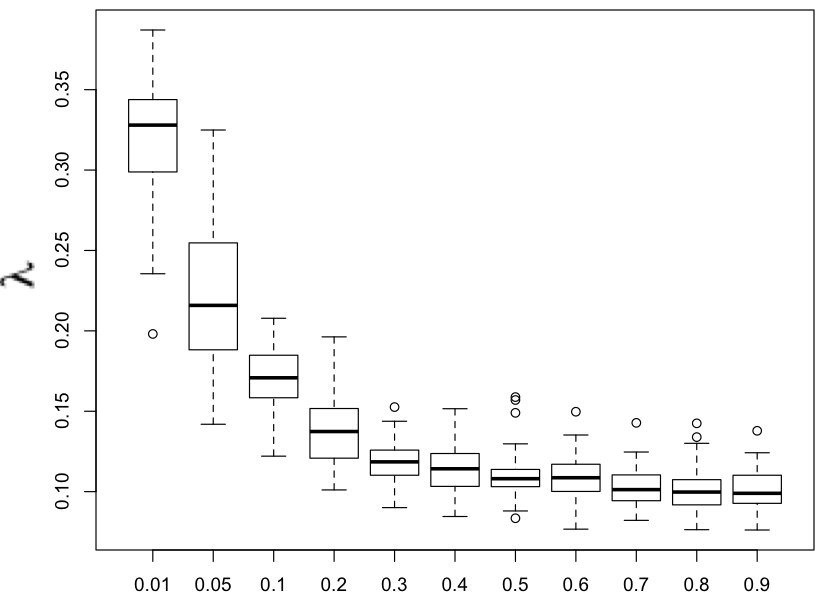
\includegraphics[width=0.4\textwidth]{50data_lambda_n_50_m1_uniform_gamadelta}
\caption{Posterior mean estimates for $\alpha$ and $\lambda^2$.}
\label{figure:m1_1}
\end{figure}

\end{frame}



\begin{frame}
\frametitle{Hydraulic application: Garonne river}
\begin{itemize}
\item TELEMAC 2D models the flow of the Garonne between Tonneins and la R\'eole:
$$
h_i = f( q_i ,\mb {K_s}),
$$
with:
\end{itemize}
\begin{minipage}{0.4\textwidth}
\begin{itemize}
\item $\mb h_i$ water heights,
\item $\mb {K_s} = ({K_s}_1,\ldots,{K_s}_5)$  Strickler coefficients (5 friction coefficients)
\item $q_i$ river flow at Tonneins
\item Linearization of the model around a reference value for the Strickler coefficient (limited to the most inflential ones).
\item Only 7 data points available.
\end{itemize}
\end{minipage}\hfill
\begin{minipage}{0.5\textwidth}
\centering{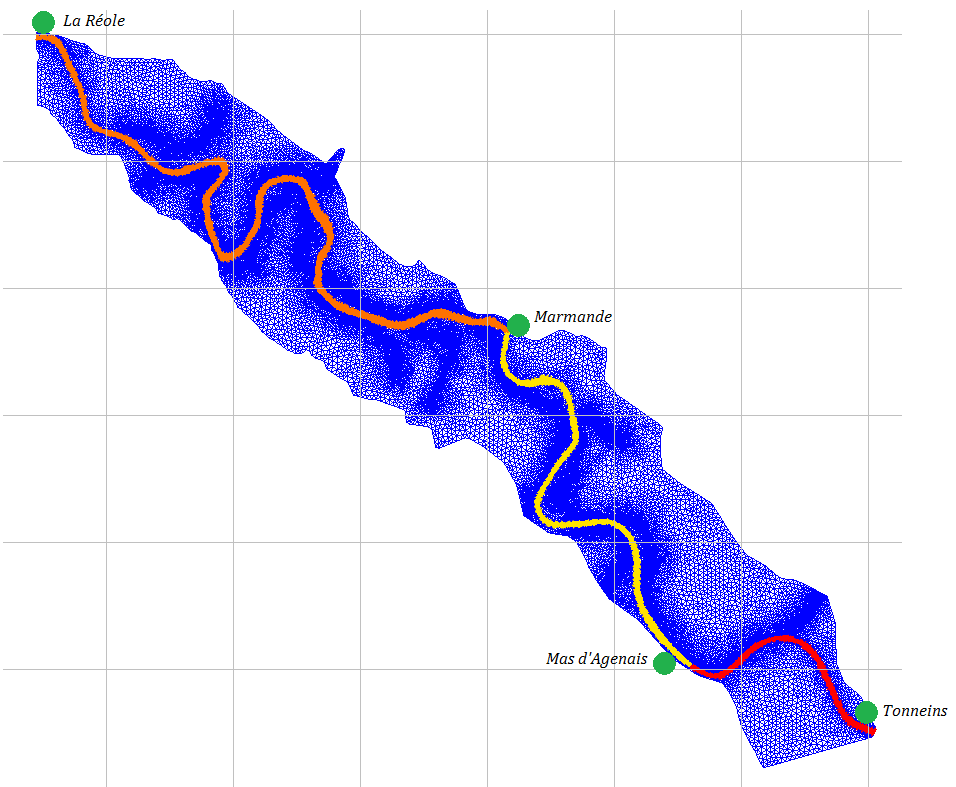
\includegraphics[width=\textwidth]{zone_frottement_garonne.PNG}}
\end{minipage}

\end{frame}


\begin{frame}
 \frametitle{Results}

 
 \begin{figure}
  \centering
  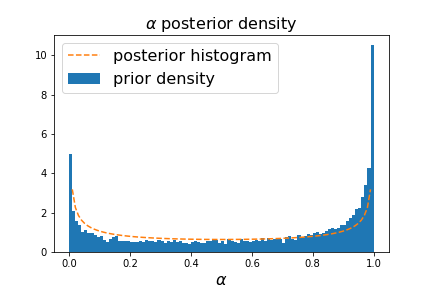
\includegraphics[scale=.3]{Marmande_Alpha_posterior_density.png}
  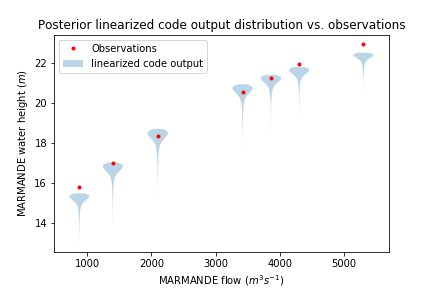
\includegraphics[scale=.3]{MARMANDE_posterior_vs_data.png}
 \end{figure}

 
 
 
 \begin{table}[h!]
\begin{tabular}{c|ccccccc}
Observation nb.		& 1		 & 2	  & 3	   & 4		& 5		 & 6	  & 7    \\ 
\hline
Bias probability &  0.513&  0.473&  0.452&  0.448&  0.451&  0.472&  0.514
\end{tabular}
\caption{\label{tab:nobias_p_Marmande} Probability of a code bias for each observation in Marmande}
\end{table}

\end{frame}




\begin{frame}
 Damblin + Kaniav
\end{frame}

\section{Variable selection}
\begin{frame}
 \frametitle{Variable Selection in the Discrepancy}
 
\end{frame}



\bibliographystyle{apalike}
\bibliography{biblio}


\end{document}
